% mnras_template.tex 
%
% LaTeX template for creating an MNRAS paper
%
% v3.0 released 14 May 2015
% (version numbers match those of mnras.cls)
%
% Copyright (C) Royal Astronomical Society 2015
% Authors:
% Keith T. Smith (Royal Astronomical Society)

% Change log
%
% v3.0 May 2015
%    Renamed to match the new package name
%    Version number matches mnras.cls
%    A few minor tweaks to wording
% v1.0 September 2013
%    Beta testing only - never publicly released
%    First version: a simple (ish) template for creating an MNRAS paper

%%%%%%%%%%%%%%%%%%%%%%%%%%%%%%%%%%%%%%%%%%%%%%%%%%
% Basic setup. Most papers should leave these options alone.
\documentclass[fleqn,usenatbib]{mnras}

% MNRAS is set in Times font. If you don't have this installed (most LaTeX
% installations will be fine) or prefer the old Computer Modern fonts, comment
% out the following line
\usepackage{newtxtext,newtxmath}
% Depending on your LaTeX fonts installation, you might get better results with one of these:
%\usepackage{mathptmx}
%\usepackage{txfonts}

% Use vector fonts, so it zooms properly in on-screen viewing software
% Don't change these lines unless you know what you are doing
\usepackage[T1]{fontenc}

% Allow "Thomas van Noord" and "Simon de Laguarde" and alike to be sorted by "N" and "L" etc. in the bibliography.
% Write the name in the bibliography as "\VAN{Noord}{Van}{van} Noord, Thomas"
\DeclareRobustCommand{\VAN}[3]{#2}
\let\VANthebibliography\thebibliography
\def\thebibliography{\DeclareRobustCommand{\VAN}[3]{##3}\VANthebibliography}


%%%%% AUTHORS - PLACE YOUR OWN PACKAGES HERE %%%%%

% Only include extra packages if you really need them. Common packages are:
\usepackage{graphicx}	% Including figure files
\usepackage{amsmath}	% Advanced maths commands
% \usepackage{amssymb}	% Extra maths symbols

%%%%%%%%%%%%%%%%%%%%%%%%%%%%%%%%%%%%%%%%%%%%%%%%%%

%%%%% AUTHORS - PLACE YOUR OWN COMMANDS HERE %%%%%

% Please keep new commands to a minimum, and use \newcommand not \def to avoid
% overwriting existing commands. Example:
%\newcommand{\pcm}{\,cm$^{-2}$}	% per cm-squared

%%%%%%%%%%%%%%%%%%%%%%%%%%%%%%%%%%%%%%%%%%%%%%%%%%

%%%%%%%%%%%%%%%%%%% TITLE PAGE %%%%%%%%%%%%%%%%%%%

% Title of the paper, and the short title which is used in the headers.
% Keep the title short and informative.
\title[New high-ionization planetary nebula]{Discovery of a new high-ionization planetary nebula in LAMOST}

% The list of authors, and the short list which is used in the headers.
% If you need two or more lines of authors, add an extra line using \newauthor
\author[Guti\'errez-Soto et al.]{
L. A. Guti\'errez-Soto,$^{1,2}$\thanks{E-mail: gsoto.angel@gmail.com}
A. N. Other,$^{2}$
Third Author$^{2,3}$
and Fourth Author$^{3}$
\\
% List of institutions
$^{1}$Instituto de Astrof\'{i}sica de La Plata (CCT La Plata - CONICET - UNLP), B1900FWA, La Plata, Argentina\\
$^{2}$Departamento de Astronomia, IAG, Universidade de S\~{a}o Paulo, Rua do Mat\~{a}o, 1226, 05509-900, S\~{a}o Paulo, Brazil\\
$^{3}$Another Department, Different Institution, Street Address, City Postal Code, Country
}

% These dates will be filled out by the publisher
\date{Accepted XXX. Received YYY; in original form ZZZ}

% Enter the current year, for the copyright statements etc.
\pubyear{2015}

% Don't change these lines
\begin{document}
\label{firstpage}
\pagerange{\pageref{firstpage}--\pageref{lastpage}}
\maketitle

% Abstract of the paper
\begin{abstract}
  We report the identification of a new planetary nebula foun in the catalog of
  emission line objects created by  \citet{Skoda:2020} based in LAMOST data...
\end{abstract}

% Select between one and six entries from the list of approved keywords.
% Don't make up new ones.
\begin{keywords}
planetary nebulae: general -- ISM: lines and bands -- surveys
\end{keywords}

%%%%%%%%%%%%%%%%%%%%%%%%%%%%%%%%%%%%%%%%%%%%%%%%%%

%%%%%%%%%%%%%%%%% BODY OF PAPER %%%%%%%%%%%%%%%%%%

\section{Introduction}

\label{sec:intro}

Planetary nebulae (PNe) represent the last stage of evolution of low- and intermediate-mass stars
(0.8$\msol$ - 8.0$\msol$). The PNe phase begin when gas is ejected from the red giant stars late
in their lives and subsequently this gas is ionized by the radiation field coming from the remnant
star resulted. An emission nebula expands, a glowing shell of ionized gas until lost in the
interstellar medium. Then the dying star core becomes a white dwarf.

The number of the PNe discovered in the galaxy is relatively low (\(\sim 3,500\)). However,
this current number of PNe represents only about 15-30\% of the estimated
total of Galactic PNe (\citealp{Frew:2008}; \citealp{Jacoby:2010}) showing that a small fraction
of the PNe have been cataloged \citep{Frew:2017}. If this is true, there will be a much larger
number of PNe in the Galaxy than if a special condition
is required. The models of \citet{Moe:2006}, for
example, predict that there are 46 000 ± 22 000 for the general case,
but only ∼6600 (De Marco & Moe 2005) if
close binaries (e.g. common-envelope phase) are required.
Miszalski et al. (2009) confirm earlier estimates that the
binary fraction of PN central stars is only 10–20\% of all
PNe, and thus, binarity is not likely to be a major factor in
the formation process. If true, there should be many PNe
waiting to be found in the Galaxy. This mean that the search for planetary nebulae
becoming a important task, that eavery time is more dificult, due to many of
the undiscovered PNe are probably
the more distant and then the more the weak. And because many of them, probably, are located
in nuvens of dust. And note that planetary nebulae only last for about 5,000-
25,000 yr \citep{Badenes:2015}, making them a very short-lived part of the stellar life cycle.
But is import to discovery new planetary nebula? the answer could be very obvious and is
related with the idea that PNe provide vital clues for the understanding late-stage stellar
evolution and Galactic chemical enrichment. Their strong emission lines allow the determination
of abundances, expansion and radial velocities, and
CSPN temperatures. The PN phase
enriches the ISM with nitrogen, carbon, helium, and dust,
important components in the formation of future generations
of stars. PNe yield information on the nuclear
burning, dredge up, and mass loss in the stellar progenitor
(see \citealp{Kwitter:2022} for an excellent recent PN
review). Thus, we need to know the number of PNe in
the Galaxy in order to develop accurate models of the
chemical enrichment rates since the initial burst of Type II
supernovae when the Galaxy was young.

PN studies have been hampered by three problems:
(i) the previous lack of accurate distances to most Galactic
PNe; (ii) obtaining representative PNe samples of the true
population diversity \citep{Parker:2022}, and (iii) their unknown
progenitor masses. The first problem has prospects of
resolution via accurate Gaia CSPN distances, though many
CSPNe remain too distant and faint for Gaia DR3 and correct
CSPN identification remains an issue for some (Parker et al.
2022). The second problem is being addressed by deep, narrow-band,
wide-field surveys, e.g., \citet{Parker:2005},
\citet{Drew:2005}, and Drew et al. (2014). For the third problem
of progenitor masses, these can only
be accurately determined for PNe in Galactic globular and
open clusters (OCs). These allow precise distance determinations
from color–magnitude diagrams (CMD) and Gaia \citep{Fragkou:2022}.

\section{Surveys}
\label{sec:surveys}
{\sc No sé si todo esto es necesario!}

\subsection{GAIA EDR3}
\label{sec:gaia}

\subsection{Pan-STARRS DR1}
\label{sec:PS1}

\subsection{LAMOST}
\label{sec:lamost}

The Large Sky Area Multi-Object Fiber Spectroscopic Telescope
(LAMOST, also named Guoshoujing Telescope) is a
telescope dedicated for spectroscopic sky survey.
There are 4000 fibers within a diameter of 1.75 meters (corresponding
to 5$^{\circ}$ in the sky) at the focal surface \citep{Cui:2012}.
The Low-Resolution Spectroscopic Survey (LRS) of LAMOST
began in October 2011, with a spectral resolving power ($R = \lambda/\Delta\lambda$)
of about 1800 and a wavelength coverage of
3700-9100~\AA \citep{Zhao:2012}. The first year observation was
for the pilot survey (Luo et al. 2012; Zhao et al. 2012),
and the regular survey began in September 2012

\section{Methodology}
\label{sec:metho}

At the beginning the idea was to identify for new planetary nebula in GAIA.
I started to constructed possibles color-color diagrams to separate PNe from
other emission lines objects and stars using GAIA only. The separation was not
good because PNe, normal stars and other emission line stars like CVs occupy the same region
in the diagram. Then, I decided to move to Pan-STARRS and combining the two
surveys Pan-STARRS and GAIA. I found one color diagram that isolate the PNe
with, I suppose, strong \ha{} emission line. By using the \((G - r)\) versus \((G_{BP} - G_{RP})\)
color-color is possible to separate those PNe excess in the in the $r$-broad-band
filter as is possible to see in the Fig~\ref{fig:gaia-ps}. Fig~\ref{fig:gaia-ps}
shows that the many of the PNe have value in the color \(G - r\) = 0, however several
PNe cover the interval in this same color between 0 and 8, and span between -1 and 5.
The orange contours represent other emission line objects that includes CV, SySt,
YSOs, AeBe stars and SNRs. The contours becoming white at the outside indicating
that the number of objects decrease significantly. And the blue contours signify
stars from \citet{Smart:2021}. Where they occupy the region with \((G - r)\) = 0.



\begin{figure}
\centering
  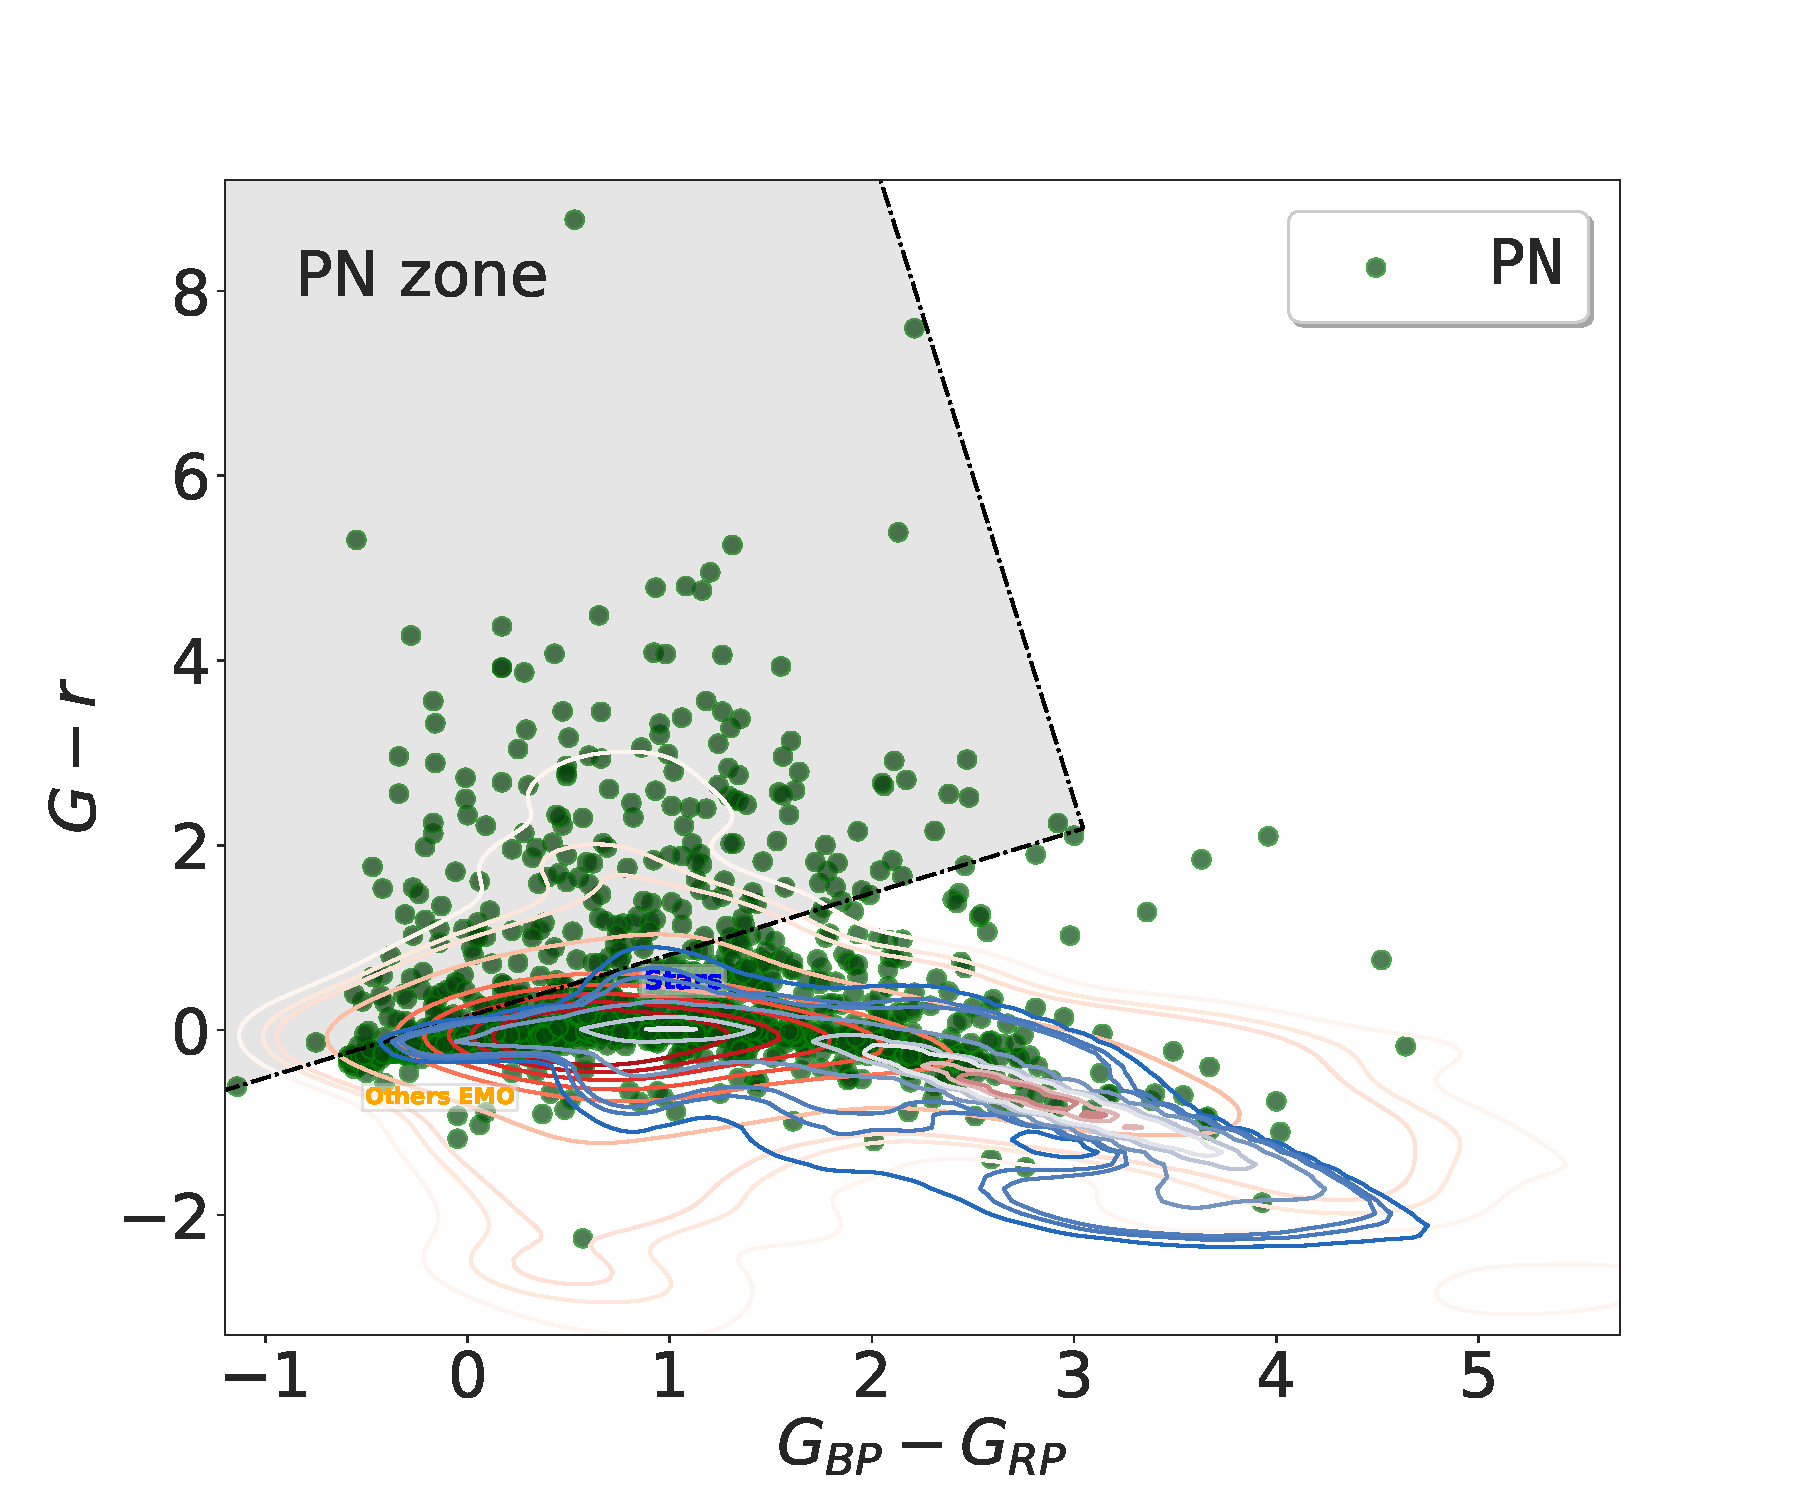
\includegraphics[width=0.9\linewidth]{Figs/color-diagram-ps-gaiaEDR3.pdf}
  \caption{} 
  \label{fig:gaia-ps}
\end{figure}

All indicate that the PNe with strong \ha{} can be selected with this color criteria??? What indicate the $G$-magnitude?.
Then, to see the possibility of using this color criterion to select these PNe, by
testing and using the emission line catalog from  \citet{Skoda:2020}. First, they
identify emission line objects from LAMOST  implementing a machine learning approach.
Then, they divided their final sample of emission line objects in tree subgroups. Those with \texttt{SIMBAD}
coincidences, those that are listed by \citet{Hou:2016} and another list that are neither cross-matched with
SIMBAD nor listed by  \citet{Hou:2016}. To texting the possibility to find for new PNe with the color criteria
explained above, we applied it directly in the new list, which present objects not reported
previously in the literature, which is a list with 1000 objects.

\begin{figure}
\centering
  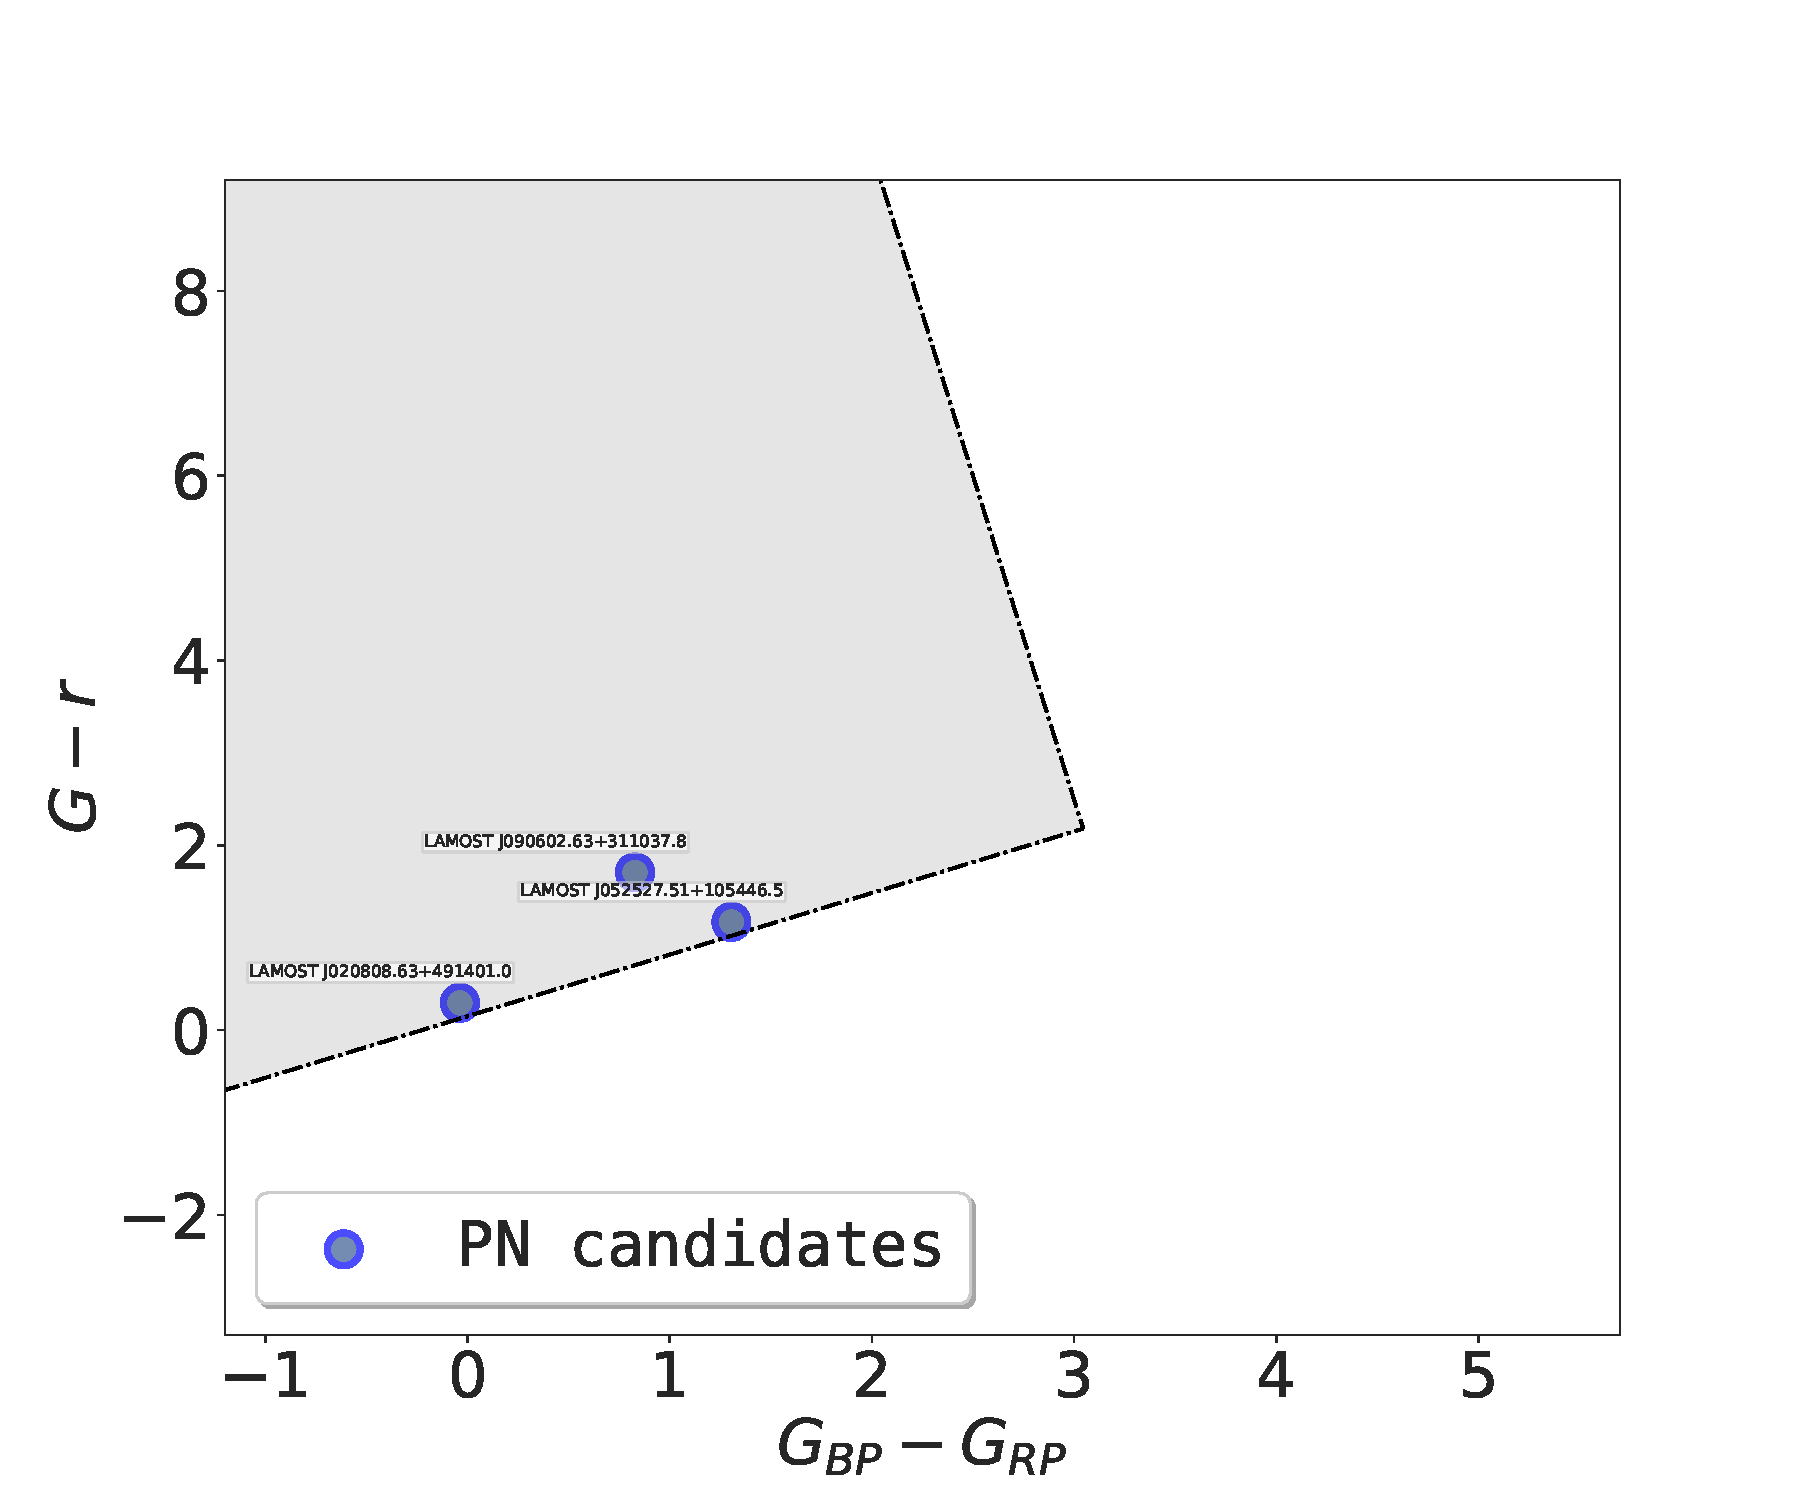
\includegraphics[width=0.9\linewidth]{Figs/pn-candidates-gaiaDR3.pdf}
  \caption{} 
  \label{fig:gaia-ps-apply}
\end{figure}

Four objects met this  condition as is possible to see in the Fig~\ref{fig:gaia-ps-apply}.
We downloaded the low resolution spectra of these objects. 
Tree objects of them display strong \ha{}, but are not display the other emission lines topically
of PNe like [O III], He II, [S II], among other. But the three look likes as PNe.
Because, it displays He II emission lines, the Balmer ones, [O III], among others.
Fig~\ref{fig:spectra} the spectrum of the new PN finding in the list of emission line of
\citet{Skoda:2020}. This PNe seem a very high ionization object, by eye is possible to see
that the He II emission line is as strong as the H$\beta$ line. No lines of ions in low stages
of ionization were detected, lines as [N II] and [O II].


Given the LAMOST spectra
are not calibrated in flux but they are flux relative, then I think that some ratio line can be calculated. Could be?

\begin{figure*}
\centering
  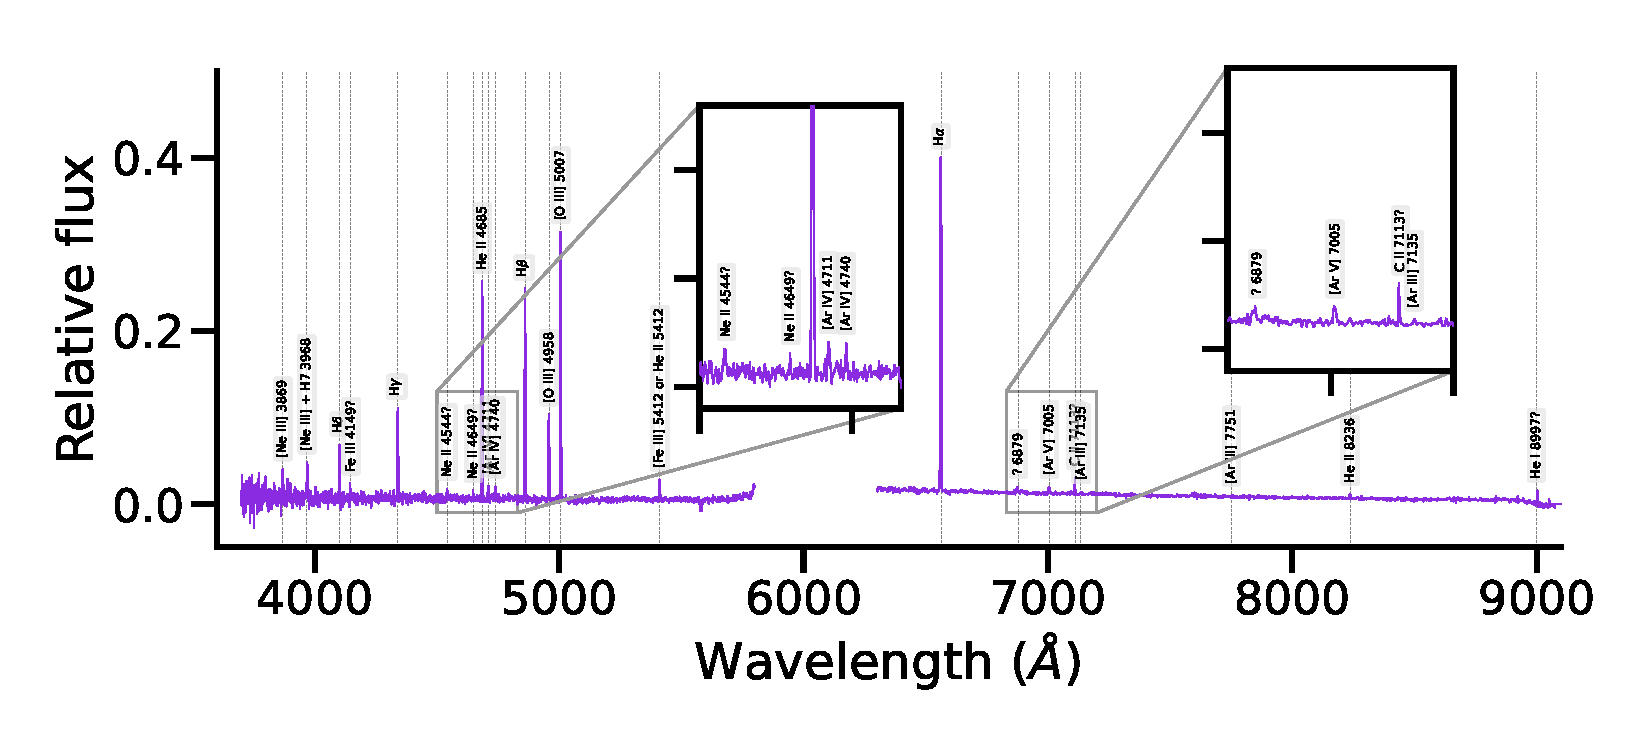
\includegraphics[width=\linewidth]{Figs/spec-56581-VB031N50V1_sp08-218.pdf}
  \caption{Low resolution spectrum from LAMOST of the new PN.} 
  \label{fig:spectra}
\end{figure*}

The images of the PN called LAMOST J020808.63+491401.0 in LAMOST are showed
in Fig~\ref{fig:image}.
\textit{Left panel} exhibits the PanSTARRS coloured
images \footnote{These RGB images were made by implementing
the python package \texttt{aplpy} \citep{aplpy:2019}}, which
was performed by combining the $g$, $r$ and $i$ filters in
the blue, green and red colour channels, respectively.
The image shows clearly a nebular component surrounding 
a central star. \textit{Right panel} shows the
WISE RGB image, with the filter W1, W2, and W4 in
the blue, green and red channels, respectively.
 The WISE image show that the object is W4 wright.
At 22$\mu$ (W4-filter) it appears as an almost
circular (but slightly elongated in the north-south direction)
diffuse halo (of angular diameter of $\simeq$ 50 arcsec) surrounding
a core of bright emission centred around J020808.63+491401.0. 


\begin{figure*}
  \centering
  \begin{tabular}{l l}
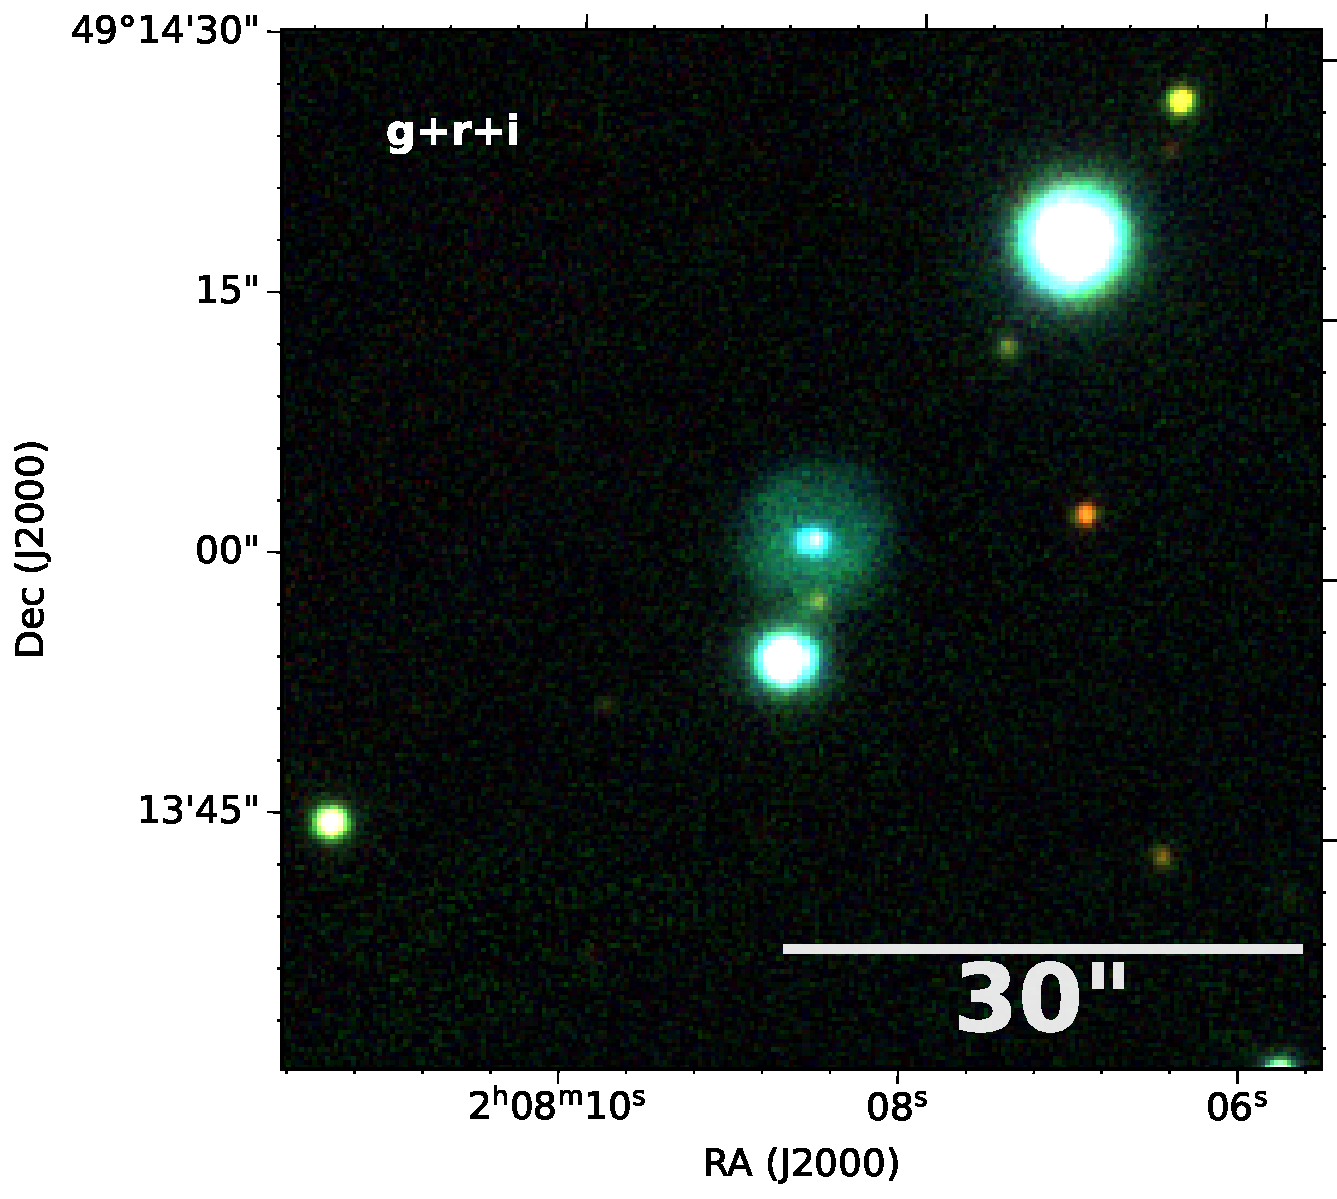
\includegraphics[width=0.5\linewidth]{Figs/cutout_rings_v3_skycell_2294_031_stk_i_unconv-irg-RGB.pdf}
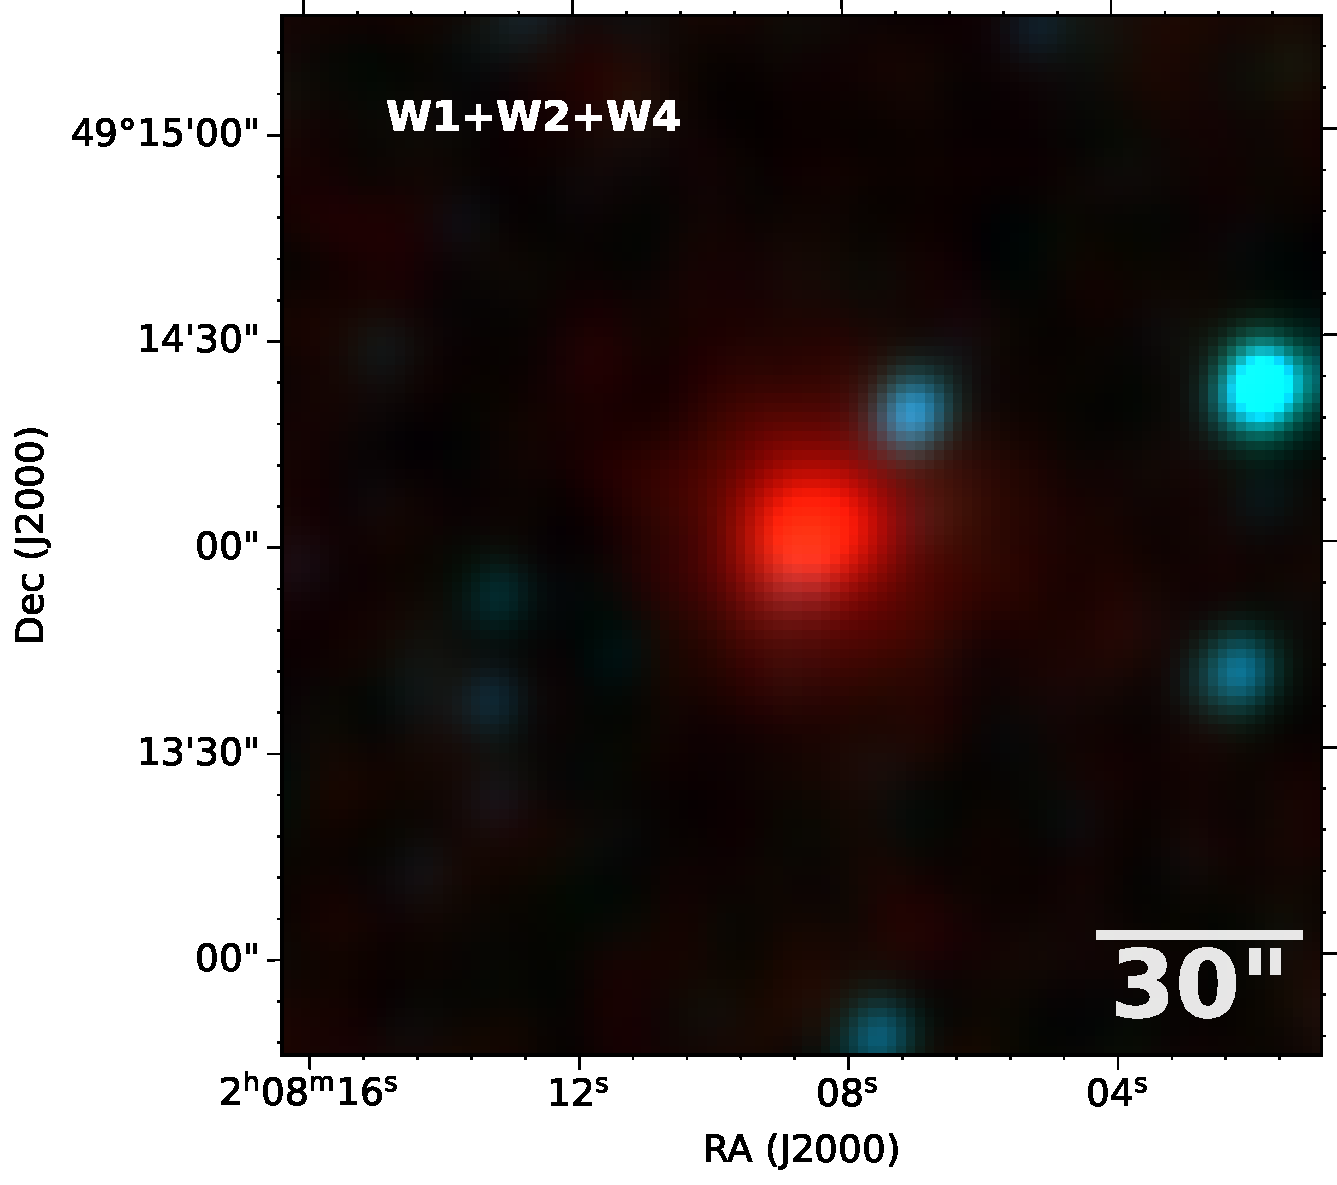
\includegraphics[width=0.5\linewidth]{Figs/w4_ra32_035994_dec49_233615-421-RGB.pdf}
\end{tabular}  
  \caption{Panstarr optical coloured image (\textit{left}) and WISE IR coloured image of the new PN. } 
  \label{fig:image}
\end{figure*}

\subsection{Why is not a supernova?}
\label{sec:snr}

Given supernovas are also high-ionization sources....

\section{Modeling the observed spectra}
\label{sec:model}

% Example table
\begin{table}
	\centering
	\caption{Best-fit {\sc cloudy} model parameters for LAMOST J020808.63+491401.0.}
	\label{tab:example_table}
	\begin{tabular}{lccr} % four columns, alignment for each
		\hline
		Parameter & Value \\
		\hline
		$\log(T_{\mathrm{BB}}) (\mathrm{K})$  & 5.146 \\
		$\log(\mathrm{luminosity) (erg~s^{-1})}$ & 37.571 \\
		  $\log(\mathrm{Hden) (cm^{-3})} $ & 3.477 \\
                  $\log(\mathrm{R_{in}) (cm)}$ & 16.903 \\
                $\log(\mathrm{R_{out}) (cm)}$ & 17.350 \\
                 Distance (pc) & 2313.01 \\
                  $\log(\mathrm{He/H})$ & -0.80 \\
                $\log(\mathrm{C/H})$ & -4.15 \\
                $\log(\mathrm{N/H})$ & -4.72 \\
                $\log(\mathrm{O/H})$ & -3.81 \\
                $\log(\mathrm{Ne/H})$ & -4.58 \\
                $\log(\mathrm{Si/H})$ & -5.00 \\
                $\log(\mathrm{S/H})$ & -6.00 \\
                $\log(\mathrm{Ar/H})$ & -6.24 \\
                
                \hline
	\end{tabular}
\end{table}

Given the small number of observational constraints, weadopt a very simple model of a planetary nebula whichconsists of a homogeneous gaseous sphere surrounding ahot star radiating as a blackbod.
Despite the LAMOST spectra are not in physical flux unity, they have flux relative. This means it
is possible compare it with other spectra in physical units. For that, I think, it is pertinent to
compare the LAMOST spectra of our PN with models.

The observed spectrum was modelled by using the {\sc cloudy} photo-ionization code version
c22.01 \citep{Ferland:2017}. This
code is based on detailed microphysics to simulate the physical
conditions of nonequilibrium gas clouds exposed to an external
radiation field. It solves the thermal, statistical, and chemical
equilibrium equations self-consistently. Currently, it uses 625
species including atoms, ions, and molecules and five distinct
databases: H-like and He-like isoelectronic sequences (Porter
et al. 2012), Stout (Lykins et al. 2015), CHIANTI (Landi et al.
2012), LAMDA (Schöier et al. 2005), and the H2 molecule
(Shaw et al. 2005) to model the spectral lines. All the known
important ionization processes, e.g., photo, Auger, collisional
and charge transfer and recombination process, namely,
radiative, dielectronic, three-body recombination, and charge
transfer are included self-consistently. {\sc cloudy} predicts both
the intensities and column densities of a very large number
(∼104) of spectral lines covering the whole electromagnetic
range, from non–local thermodynamic equilibrium (NLTE),
illuminated gas clouds by solving the equations of thermal and
statistical equilibrium for a given set of input parameters. More
details about CLOUDY could be found in Ferland et al. (2013);
Shaw et al. (2020), and references therein (Pandey et al. 2022).
In the past, \citet{Vejar:2019} used {\sc cloudy} to produce
synthetic spectra of PNe to simulate the  Broadband photometry
of Large Synoptic Survey Telescope(LSST). In the same way, a grid of modelled
halo galactic PNe were performed to simulate the J-PLUS and S-PLUS photometry
to developed new color criteria to find for PNe in these surveys by \citet{Gutierrez-Soto:2020}.
We used {\sc pyCloudy} \citep{Morisset:2013} a package python\footnote{\url{https://sites.google.com/site/pycloudy/home}} which is a set of tools to deal with photoionization code {\sc cloudy} (\url{www.nublado.org}), which was used to create a set of input of model and lead with the  output files.


The code uses a set of input parameters to compute the
ionization, thermal, and chemical state of a non-equilibrium gas cloud, illuminated
by a central source and predict the resulting spectra. 


Fig~\ref{fig:spectra-obs-model} shows a comparison
between LAMOST spectra and a {\sc cloudy} modelled spectra from \citet{Gutierrez-Soto:2020}.
Note that only is an example for illustrative intentions. This model was taken from a grid of
models that reproduce spectra form the Galactic halo. For this, it don't exist a real matches between
the two spectra. I will a perform a grid of PN models that better reproduce the LAMOST spectra of our candidate.
However, almost all the line are reproduce with this model, that could be interesting, because the
temperature effective of this model is 130$\times10^3$K, indicating a very high excitation object.
Maybe, it will be good idea estimate ratio lines to confirm that! is it possible with this spectrum?
The observed spectrum and the modeled spectrum were
matched using fluxes relative to the H{$\beta$} emission line.



\begin{figure*}
\centering
  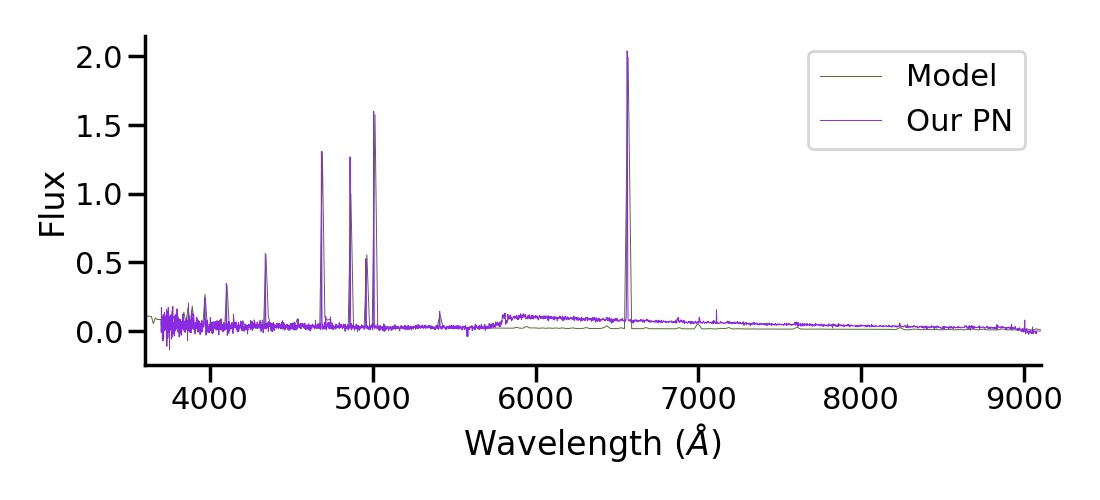
\includegraphics[width=0.89\linewidth]{Figs/model_140000_37.57.jpg}
  \caption{} 
  \label{fig:spectra-obs-model}
\end{figure*}

\section{Comparing with other high-ionization PNe. }
\label{sec:comp}

\newpage
\begin{figure*}
\centering
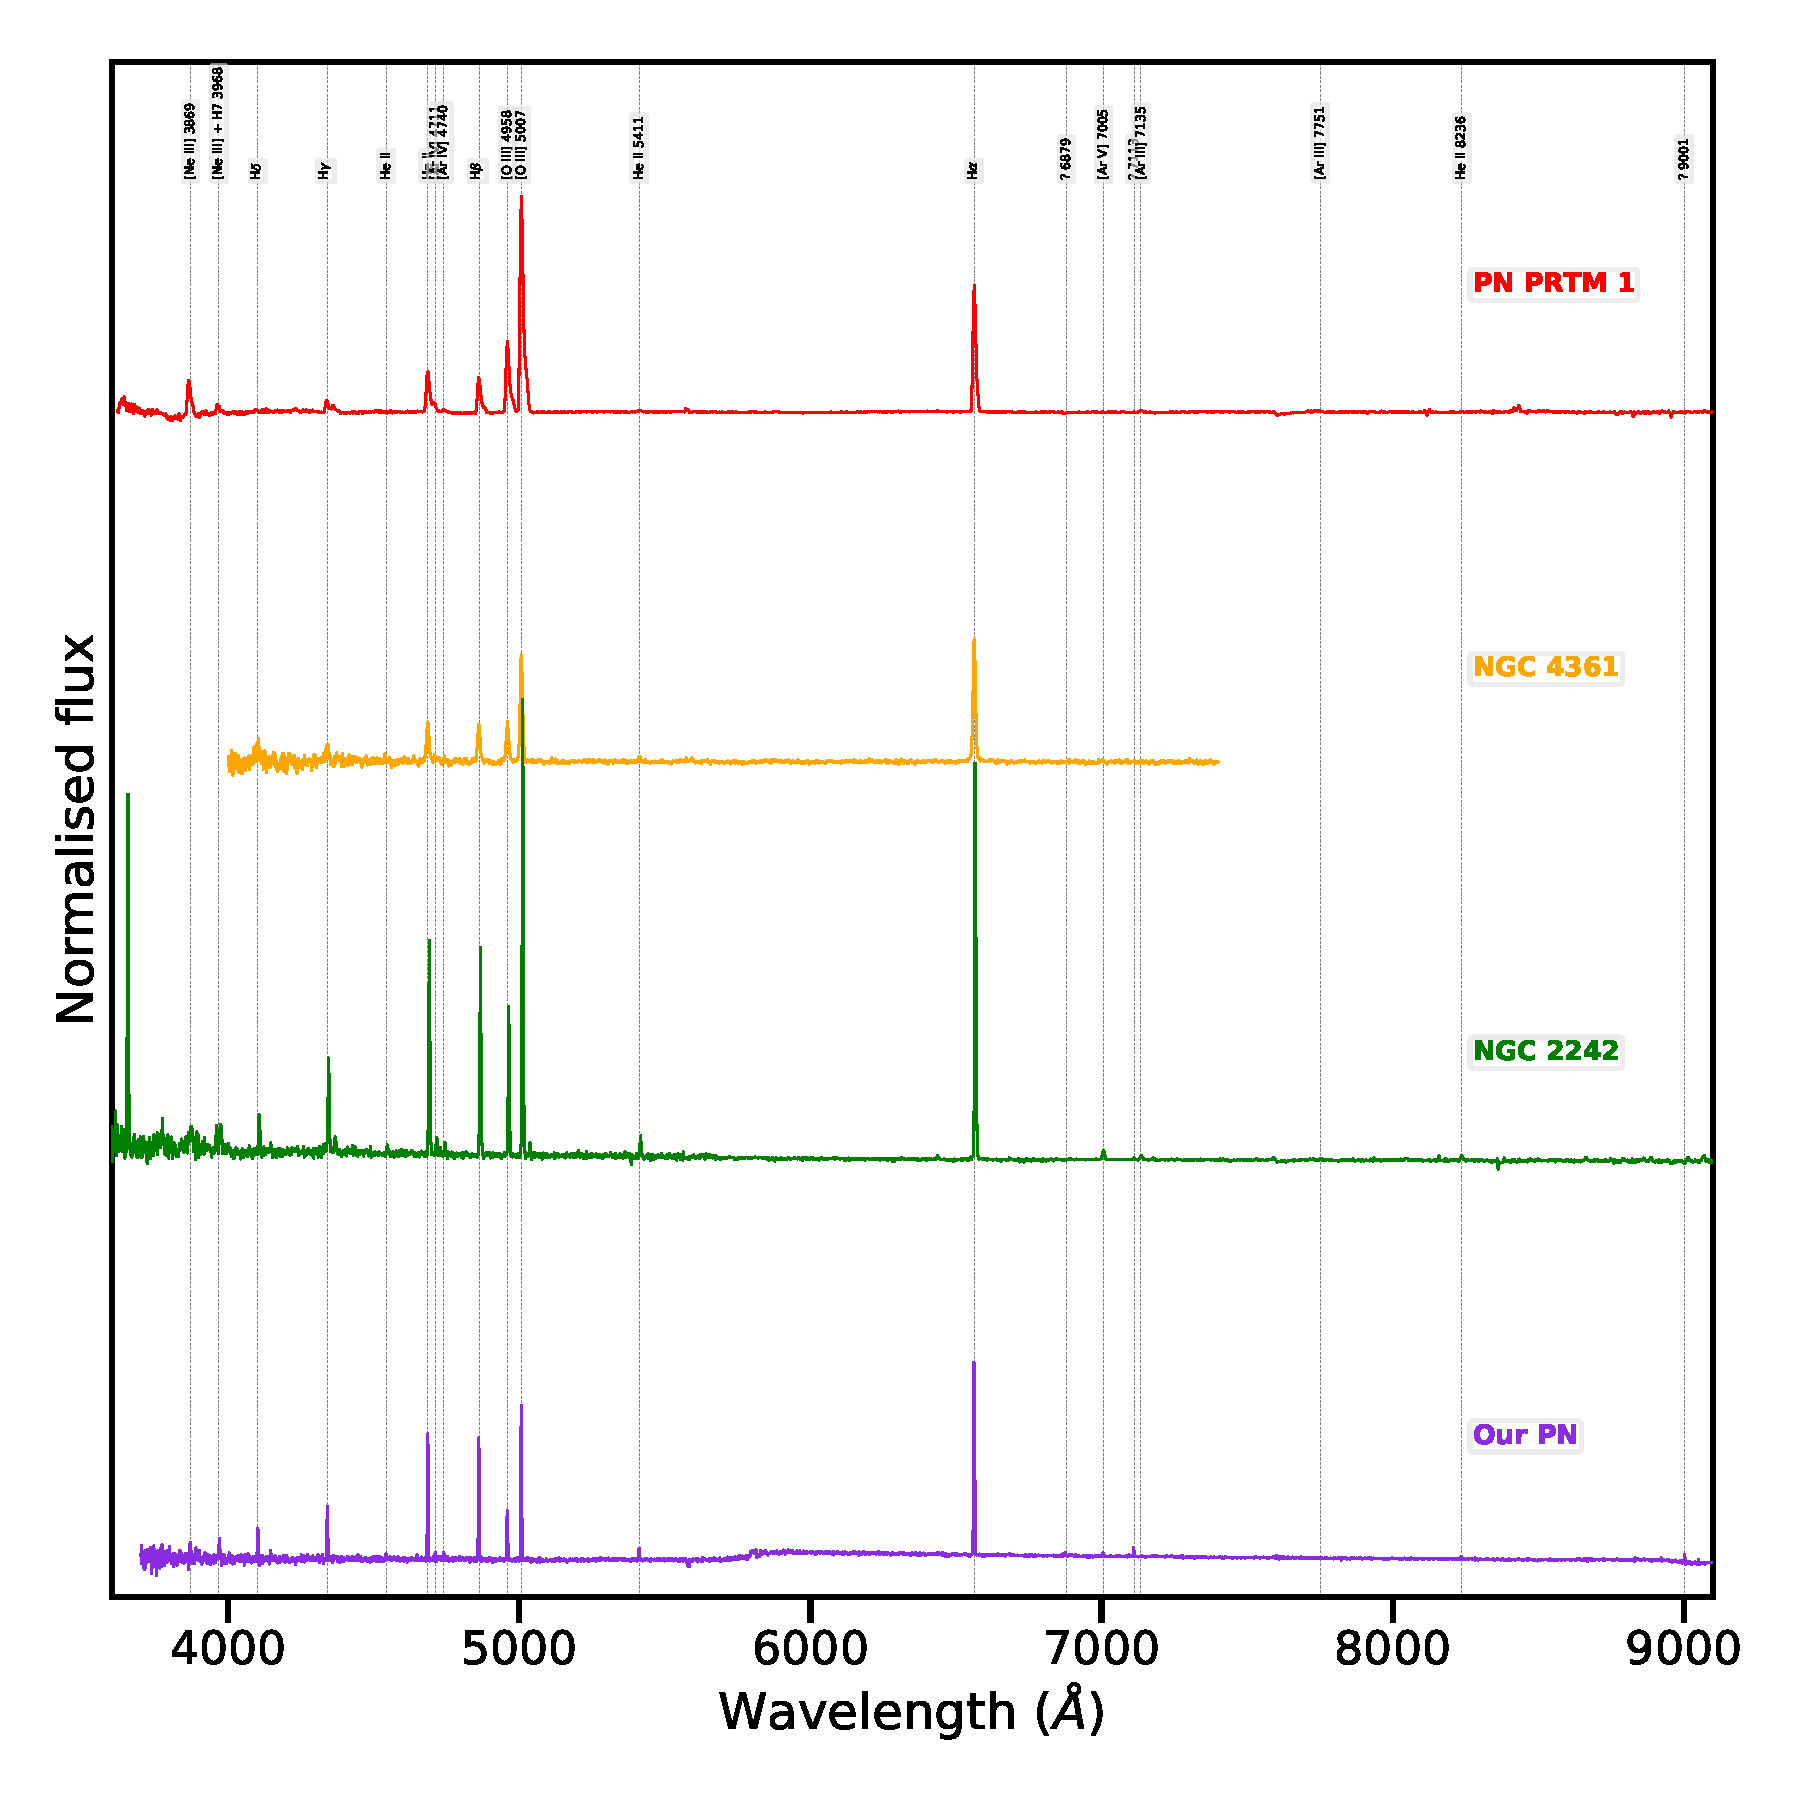
\includegraphics[width=0.89\linewidth]{Figs/spectra-compare.pdf}
  \caption{Comparing the new PNe with other high halo palnetary nebulae... The spectra were normalised to H{$\beta$}.} 
  \label{fig:compare-spectra}
\end{figure*}

In Fig~\ref{fig:compare-spectra} we are compare our PNe with other high-ionization PNe (NGC 2242, NGC 4361 and PRTM 1). Note that all three PNe are objects located at high latitudes, this means that they belong to the halo Galactic. All four spectra are very similar with the same Balmer lines, the high-ionization lines and lacked the low-ionization lines.

\begin{figure}
  \centering
  \begin{tabular}{l l}
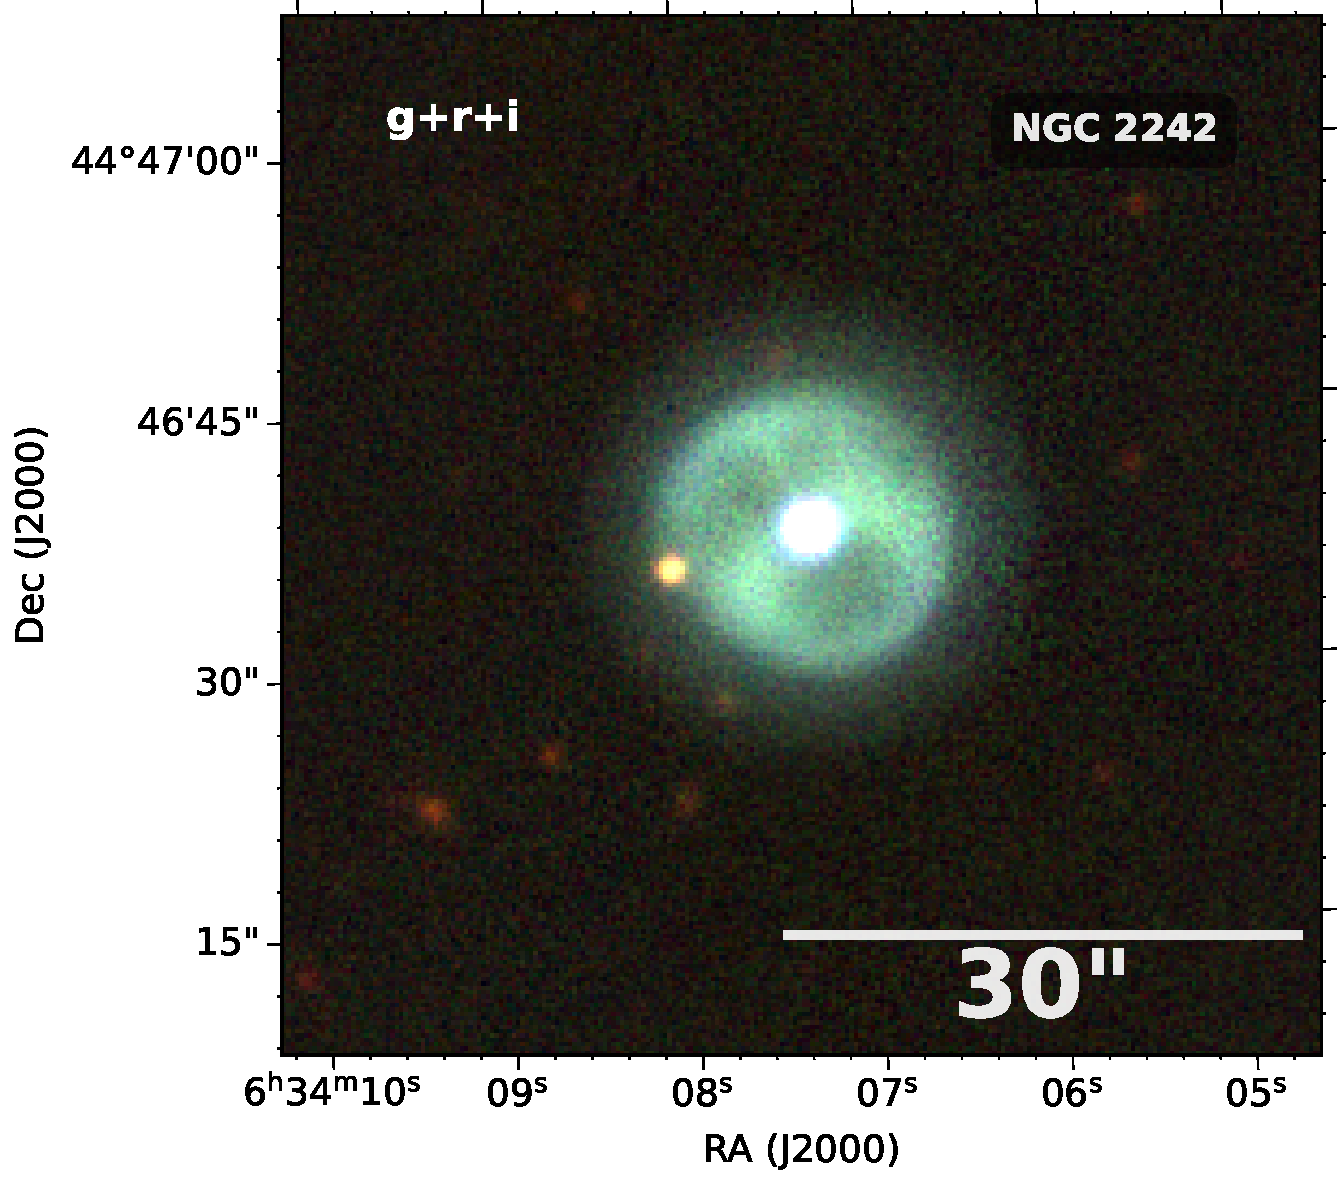
\includegraphics[width=0.52\linewidth]{Figs/cutout_rings.v3.skycell.2243.029.stk.i.unconv-irg-RGB.pdf}
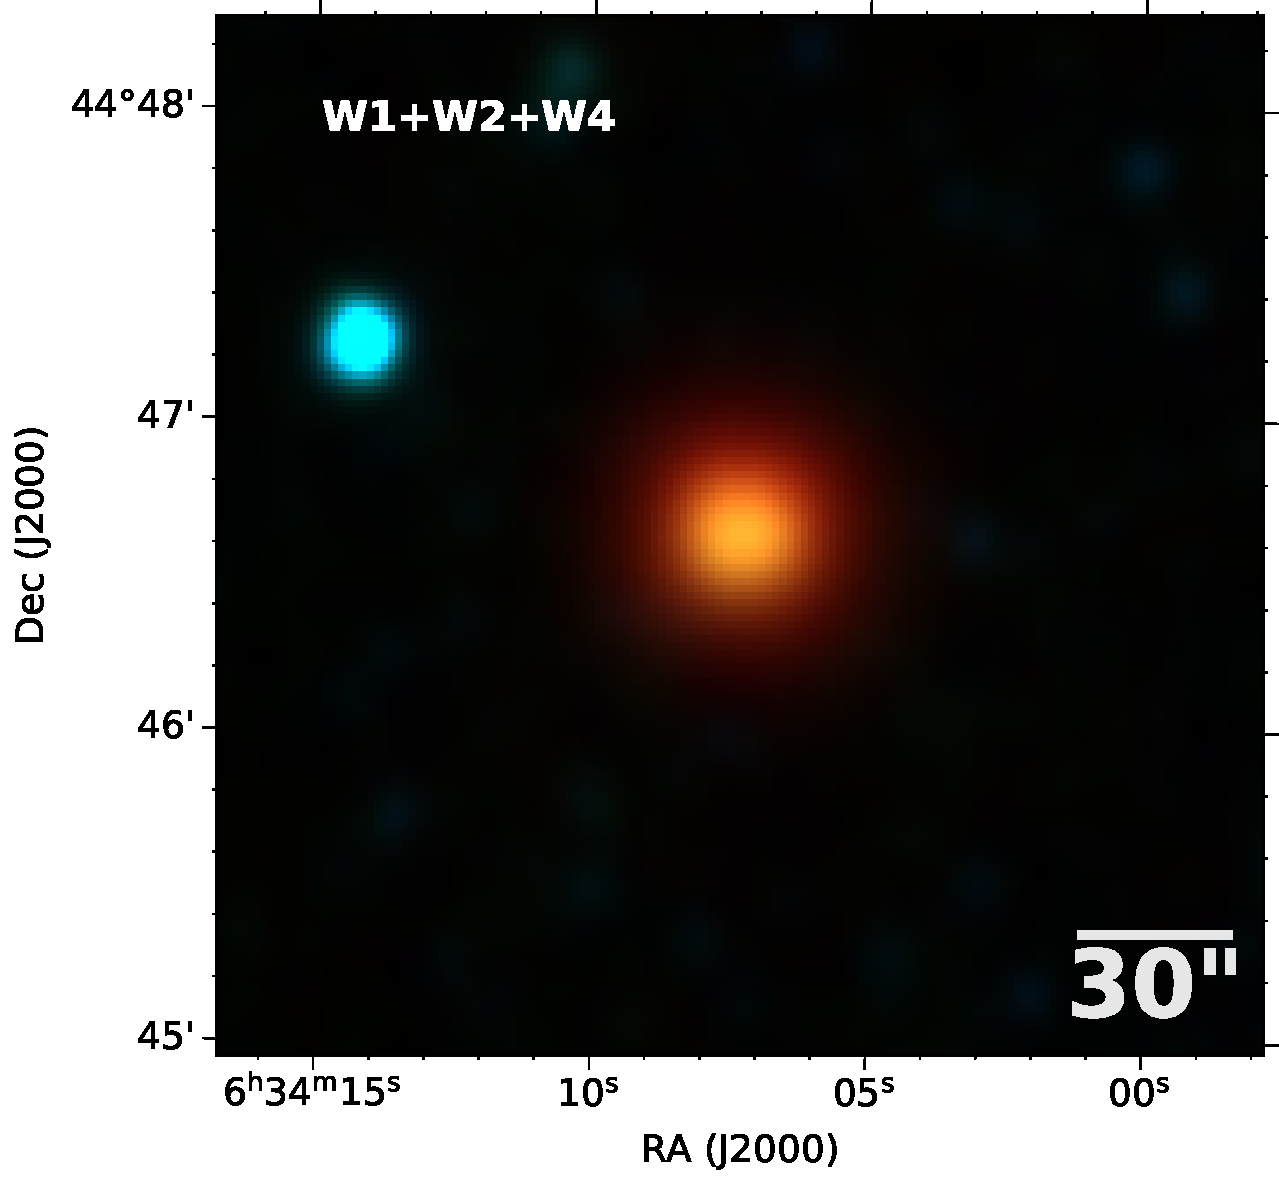
\includegraphics[width=0.5\linewidth]{Figs/0979p454_ac51-w4-int-3_ra98.53061791727998_dec44.77716333248_asec200.000-421-RGB.pdf}\\
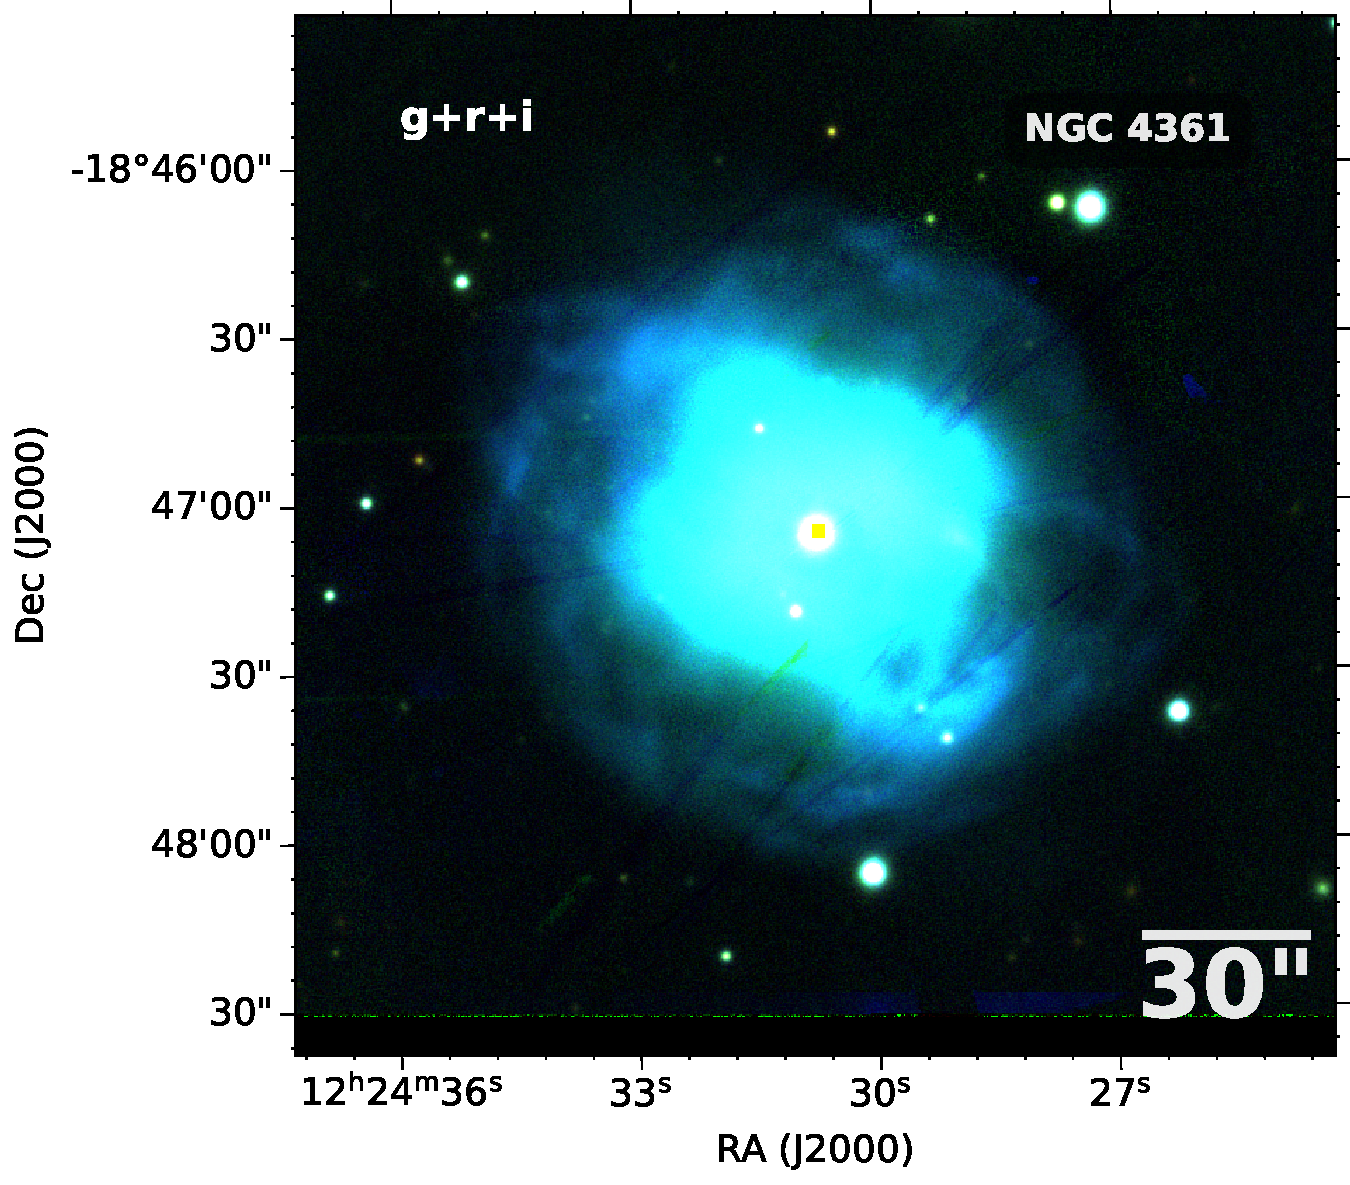
\includegraphics[width=0.52\linewidth]{Figs/cutout_rings.v3.skycell.0924.030.stk.i.unconv-irg-RGB.pdf}
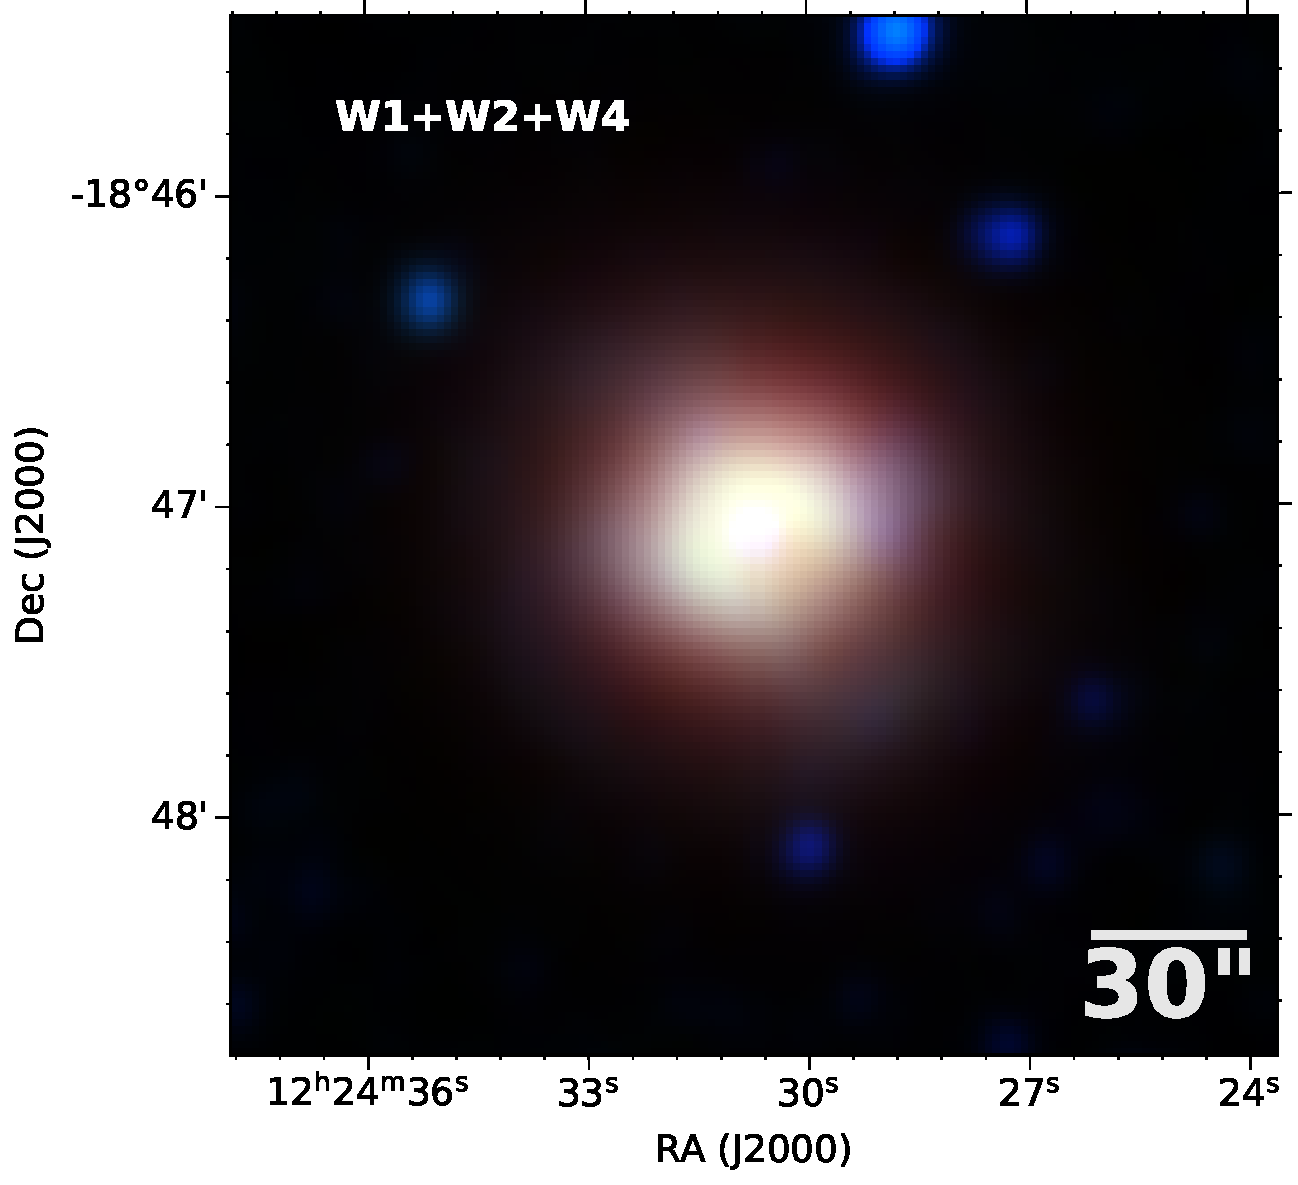
\includegraphics[width=0.5\linewidth]{Figs/1855m182_ac51-w4-int-3_ra186.12812938647002_dec-18.78487981564_asec200.000-421-RGB}\\
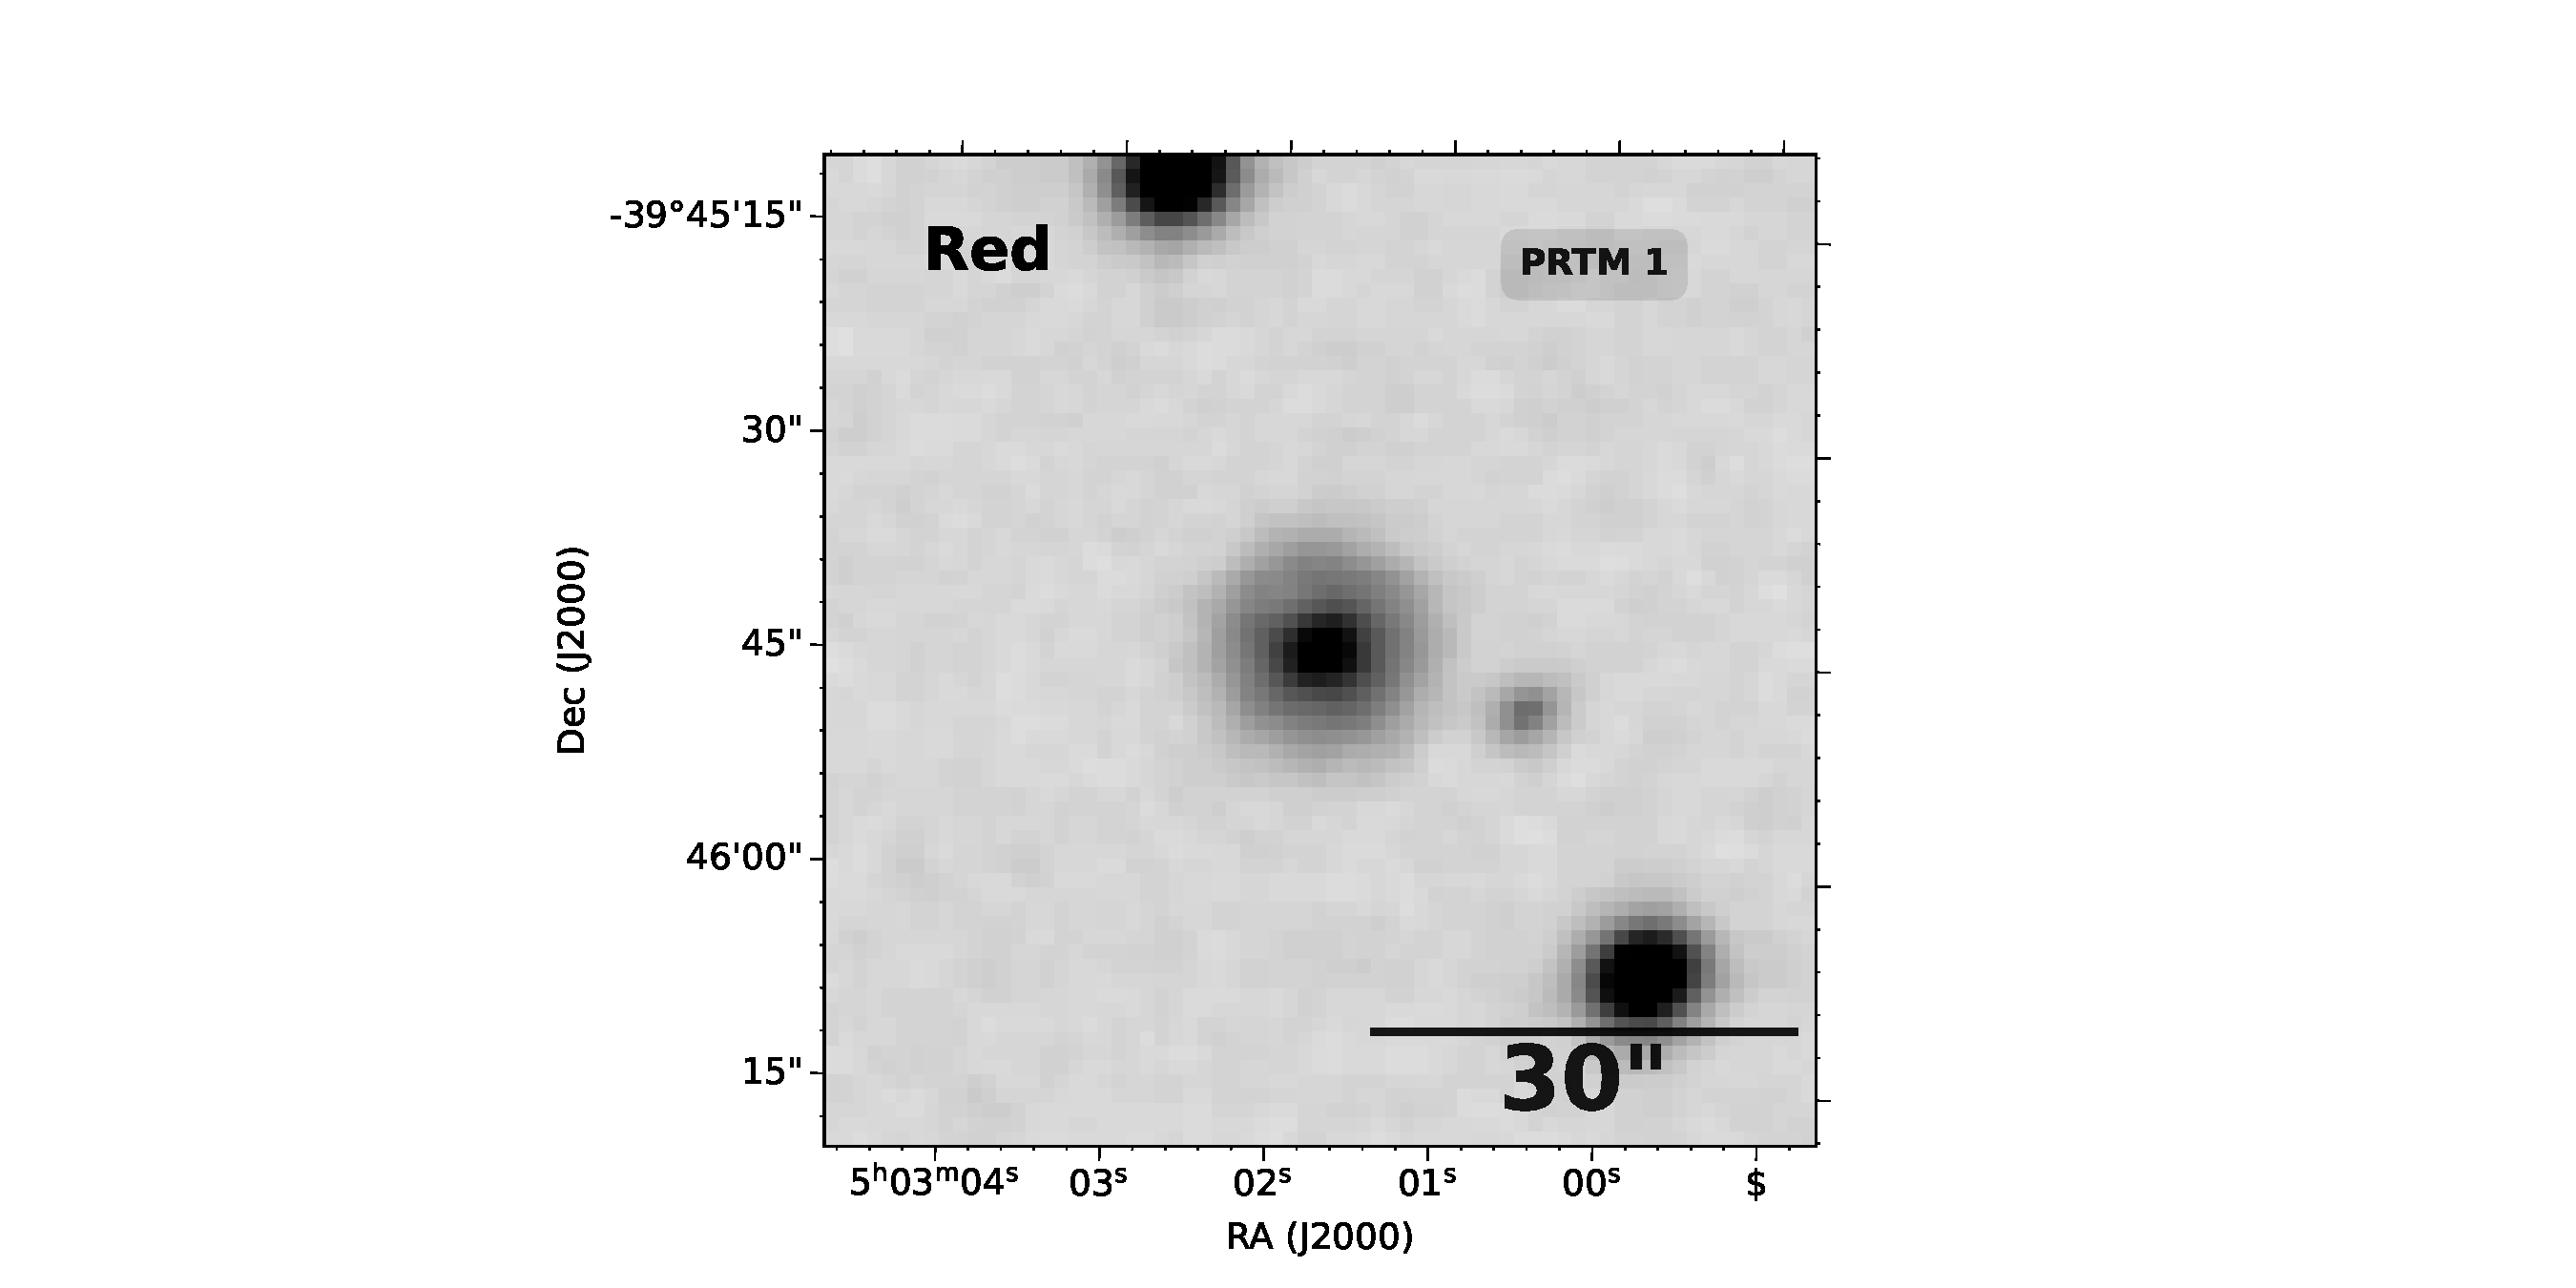
\includegraphics[width=0.535\linewidth, trim=280 10 340 10, clip]{Figs/dss_search_red.pdf}
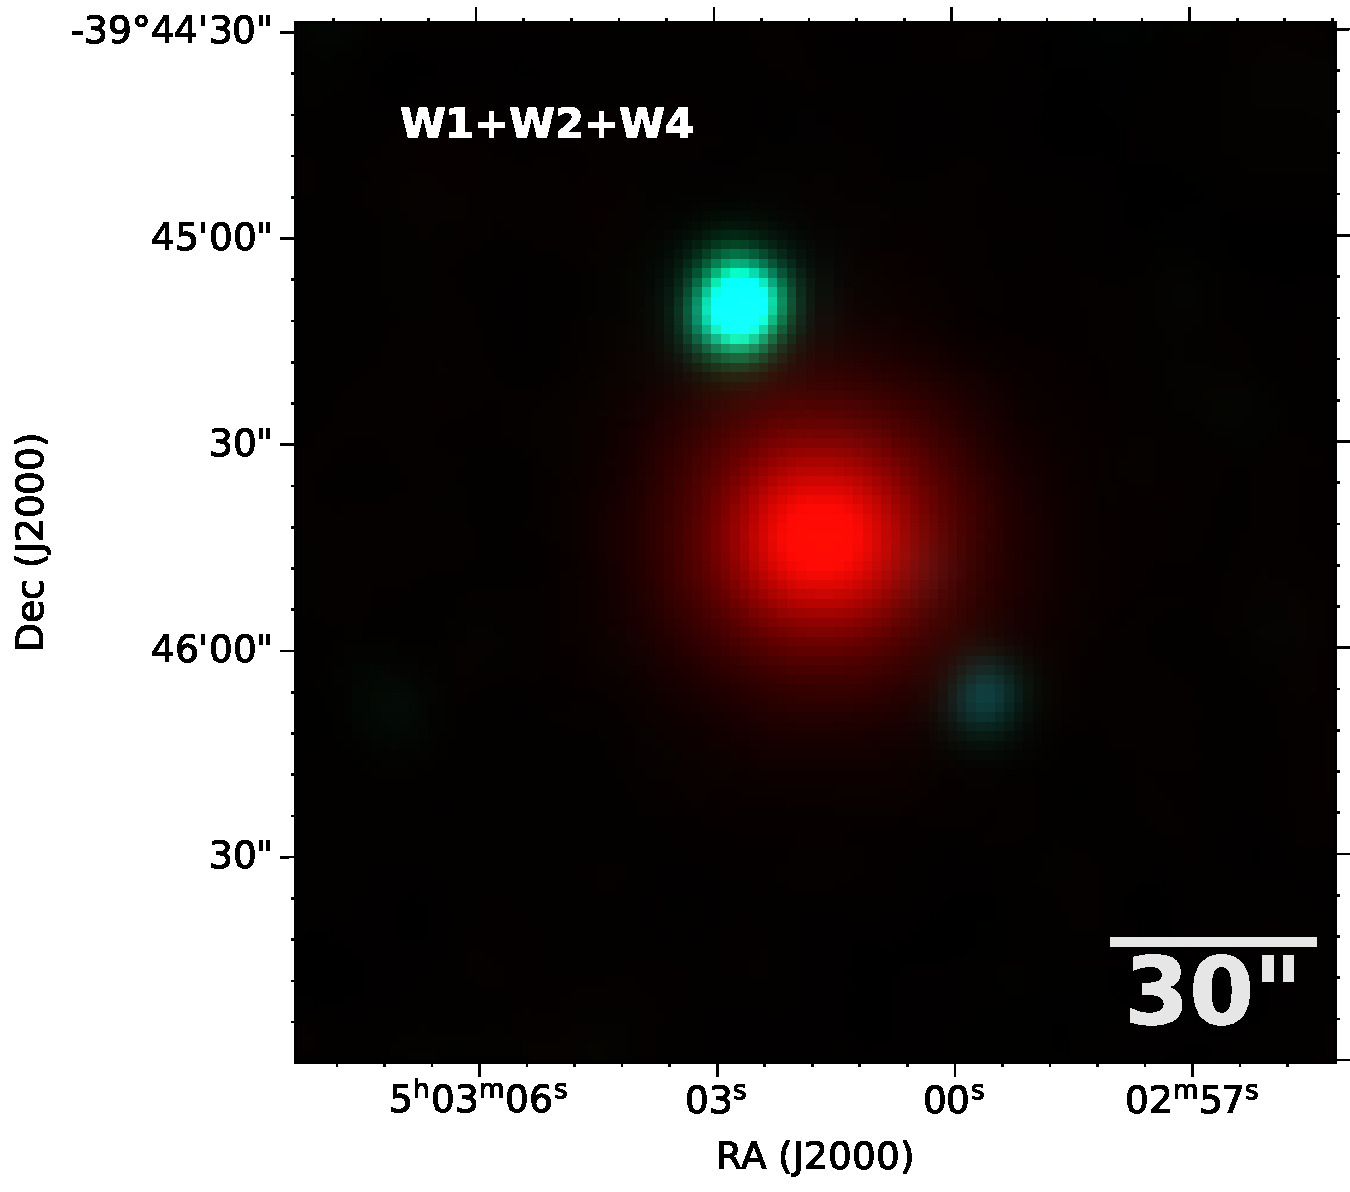
\includegraphics[width=0.47\linewidth, trim=58 0 0 0]{Figs/0754m394_ac51-w4-int-3_ra75.75721626934_dec-39.76236833917_asec150.000-421-RGB.pdf}\\

\end{tabular}  
  \caption{Optical (\textit{right}) and IR (\textit{left}) images of the other high-ionization PNe.. For comparison. } 
  \label{fig:images-known}
\end{figure}

Fig~\ref{fig:images-known}

\section{Comparison with post-AGB stellar evolution tracks}
\label{sec:tracks}

\begin{figure}
\centering
  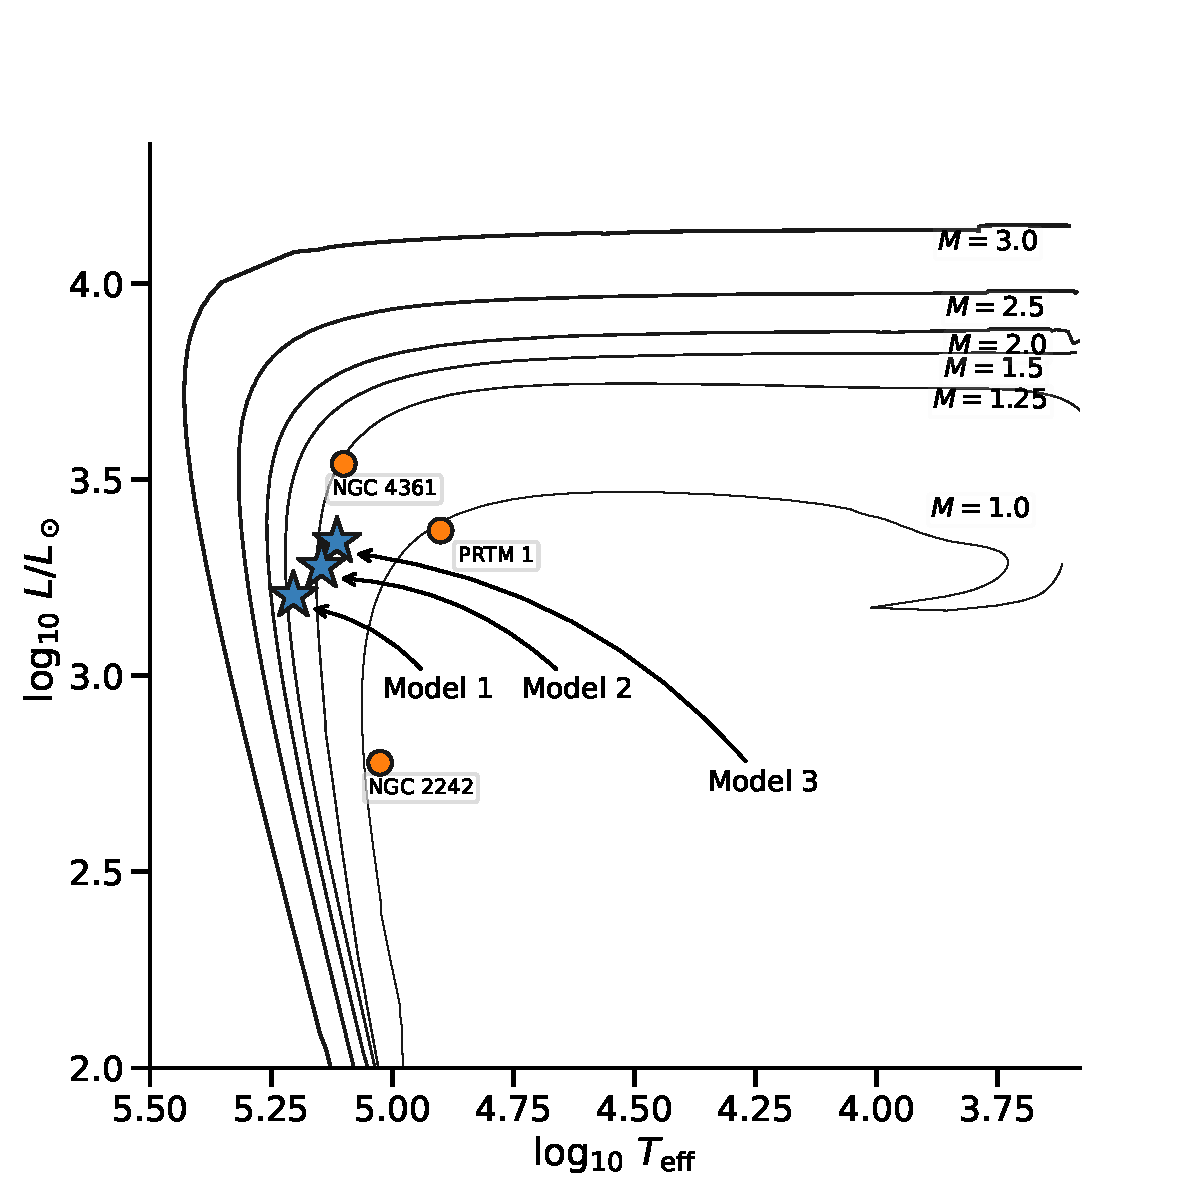
\includegraphics[width=\linewidth]{Figs/hr-planetarieNebula}
  \caption{HR diagram of PN central stars, showing the observed luminosity
and effective temperature of the new PN, compared with
post-AGB evolutionary tracks from \citet{Miller:2016} (solid lines,
labelled with initial stellar mass in solar masses). Small star symbols show
an evolutionary time along each track equal to the kinematic age of the
intermediate shell of NGC 2242, with blue shading indicating 50 per cent
variation about this value.  Filled symbols shows the known PN showed in section~\ref{}
that have been selected to be  similar to the new PNe. {\sc Ok! falta colocar la nueva nebulosa}.} 
 \label{fig:track-evolutive}
\end{figure}

Fig~\ref{fig:track-evolutive} shows... Post-AGB stellar evolutionary tracks for
approximately solar metallicity \citep{Miller:2016} are indicated

\section*{Acknowledgements}

The Acknowledgements section is not numbered. Here you can thank helpful
colleagues, acknowledge funding agencies, telescopes and facilities used etc.
Try to keep it short.

%%%%%%%%%%%%%%%%%%%%%%%%%%%%%%%%%%%%%%%%%%%%%%%%%%
\section*{Data Availability}

 
The inclusion of a Data Availability Statement is a requirement for articles published in MNRAS. Data Availability Statements provide a standardised format for readers to understand the availability of data underlying the research results described in the article. The statement may refer to original data generated in the course of the study or to third-party data analysed in the article. The statement should describe and provide means of access, where possible, by linking to the data or providing the required accession numbers for the relevant databases or DOIs.


%%%%%%%%%%%%%%%%%%%% REFERENCES %%%%%%%%%%%%%%%%%%

% The best way to enter references is to use BibTeX:

\bibliographystyle{mnras}
\bibliography{Ref-pne} % if your bibtex file is called example.bib


% Alternatively you could enter them by hand, like this:
% This method is tedious and prone to error if you have lots of references
%\begin{thebibliography}{99}
%\bibitem[\protect\citeauthoryear{Author}{2012}]{Author2012}
%Author A.~N., 2013, Journal of Improbable Astronomy, 1, 1
%\bibitem[\protect\citeauthoryear{Others}{2013}]{Others2013}
%Others S., 2012, Journal of Interesting Stuff, 17, 198
%\end{thebibliography}

%%%%%%%%%%%%%%%%%%%%%%%%%%%%%%%%%%%%%%%%%%%%%%%%%%

%%%%%%%%%%%%%%%%% APPENDICES %%%%%%%%%%%%%%%%%%%%%

\appendix

\section{Some extra material}

If you want to present additional material which would interrupt the flow of the main paper,
it can be placed in an Appendix which appears after the list of references.

%%%%%%%%%%%%%%%%%%%%%%%%%%%%%%%%%%%%%%%%%%%%%%%%%%


% Don't change these lines
\bsp	% typesetting comment
\label{lastpage}
\end{document}

% End of mnras_template.tex
